\section{\sysname: Design and Implementation}
\label{sec:design}

Our primary observation is that \textit{physical memory fragmentation can be avoided without making \kvcache non-contiguous in virtual memory.} To realize this, \sysname decouples the allocation of virtual memory from physical memory by leveraging system support for demand paging (instead of implementing demand paging in user space, as in \pa). 

%Our goal is to avoid fragmentation in \textbf{physical} memory without making \kvcache non-contiguous in \textbf{virtual} memory. To achieve this goal, \sysname leverages system support for demand paging instead of implementing it in user space. 


\subsection{Design Overview}
\label{sec:design:overview}

\sysname employs distinct allocation policies for virtual and physical memory. Specifically, we allocate a large contiguous buffer for the \kvcache in virtual memory ahead-of-time (similar to systems prior to \pa) while deferring the allocation of physical memory to runtime (similar to \pa). This design preserves virtual contiguity of \kvcache without fragmenting physical memory. Note that this approach could fragment and waste virtual memory. However, this is not an issue since virtual memory is abundant, e.g., modern 64-bit systems provide a 128TB user-addressable virtual memory per  process.\footnote{64-bit systems use only 48 bits for virtual addresses today, providing a per-process virtual memory space of 256TB which is divided equally between the user space and (OS) kernel space.}




\subsubsection{Pre-reserving virtual memory}
Since virtual memory is abundant, we pre-allocate it in size that is large enough to hold the \kvcache of the maximum batch size (configurable) that needs to be supported. In doing so, we assume that each request's context length is same as the maximum  supported by the model.

\subsubsection{Number of virtual memory buffers}
A serving framework maintains separate K and V tensors for each layer of the model. Therefore, we reserve $2\times N$ buffers on a worker where $N$ is the number of layers managed by that worker. %In a multi-GPU job, a worker may host only a subset of the layers of the model.  by that worker ($N^\prime=N$ with tensor-parallelism whereas $N^\prime < N$ with pipeline-parallelism).

%For a single GPU job, this requires pre-reserving $2\times N$ buffers where $N$ is the number of layers in the model. In a multi-GPU job, each worker reserves $2\times N^\prime$ buffers where $N^\prime$ is the number of layers managed by that worker ($N^\prime=N$ with tensor-parallelism whereas $N^\prime < N$ with pipeline-parallelism).

\begin{table*}[t!]
    \centering
    \scalebox{0.85}{
    \begin{tabular}{l|l|l|c|c|c|c}
    & & & \multicolumn{4}{c}{\textbf{Latency (microseconds)}} \\ 
       \textbf{CUDA VM APIs} & \textbf{\sysname VM APIs} & \textbf{Description} & \textbf{64KB} & \textbf{128KB} & \textbf{256KB} & \textbf{2MB} \\ \toprule
      \cumemreserve*  & \vmemreserve*    & Allocate a buffer in virtual memory          & 18 & 17 & 16 & 2     \\
      \cumemcreate*   & \vmemcreate*     & Allocate a handle in physical memory         & 1.7 & 2  & 2.1 & 29      \\
      \cumemmap       & \vmemmap         & Map a physical handle to a virtual buffer      & 8 & 8.5 & 9 & 2      \\
      \cumemsetaccess & -                    & Enable access to a virtual buffer         & - & - & - & 38       \\ \hdashline 
      \cumemunmap     & -                    & Unmap physical handle from a virtual buffer  & - & - & - & 34       \\
      \cumemrelease*  & \vmemrelease*    & Free physical pages of a handle             & 2 & 3 & 4 & 23       \\
      \cumemfree*     & \vmemfree*       & Free a virtual memory buffer                 & 35 & 35 & 35 & 1        \\
      \bottomrule
    \end{tabular}}
    \caption{CUDA VMM APIs. * represents APIs that we use once while instantiating or terminating the serving framework. Rest of the APIs are used for (un)mapping physical memory pages at runtime. CUDA APIs (prefixed with cu) support only 2MB pages, whereas our CUDA extension APIs (prefixed with v) support fine-grained allocations.}
    \label{tab:design:cudaapis}
\end{table*}


\subsubsection{Size of a virtual memory buffer}
\label{sec:design:buffersize}
The maximum size of a buffer is $BS=B\times S$ where B is the maximum batch size and $S$ is the maximum size of a single request's per-layer \kcache (or \vcache) on a worker. Further, $S=L\times H\times D\times P$, where $L$ is the maximum context length supported by the model, $H$ is the number of KV heads on a worker, $D$ is the dimension of each KV head and $P$ is the number of bytes based on model precision (e.g., P=2 for FP16/BF16).  As an example, consider \yimedium with FP16 and two-way tensor-parallelism (TP-2). In this case, $N\!=\!60, H=4, D=128, P=2$ (8 KV heads of \yimedium are split evenly on two GPUs), and maximum supported context length $L=200K$. For this configuration, $S=200MB$ $(200K*4*128*2)$. Assuming $B=500$, the maximum size of each buffer per-worker is $BS=100GB$ ($500\times 200MB$). Therefore, the total virtual memory requirement for 60 layers is 120 buffers of 100GB each (12TB total). Note that the size of virtual address space available grows with the number of workers, e.g., with two TP workers, the total size of user-addressable virtual address space is 256TB. Therefore, virtual memory is always plentiful to satisfy large allocations. \autoref{fig:design:vattention} shows an example of how \sysname allocates physical memory pages dynamically.



\subsection{Leveraging CUDA Virtual Memory Support}

The standard GPU memory allocation interface \cudamalloc does not support demand paging, i.e., it allocates virtual memory and physical memory at the same time. However, recent CUDA versions provide programmers a fine-grained control over managing virtual and physical memory, including support for decoupling their allocations~\cite{cudavirtualmemory, gmlakeasplos24}. We leverage these low-level APIs.

\subsubsection{CUDA virtual memory APIs}~\autoref{tab:design:cudaapis} provides an overview of CUDA VMM APIs that allow decoupling the allocation of virtual memory from physical memory. The allocation granularity depends on the page size used by the GPU. Further, the size of a virtual memory buffer or a physical memory handle must be a multiple of the physical memory allocation granularity.  Physical memory pages can be allocated to (or de-allocated from) sub-regions in a virtual memory buffer independently of other sub-regions. 

%For simplicity, we refer to the granularity of physical memory allocation as \textit{page size}.
\begin{figure}
    \centering
    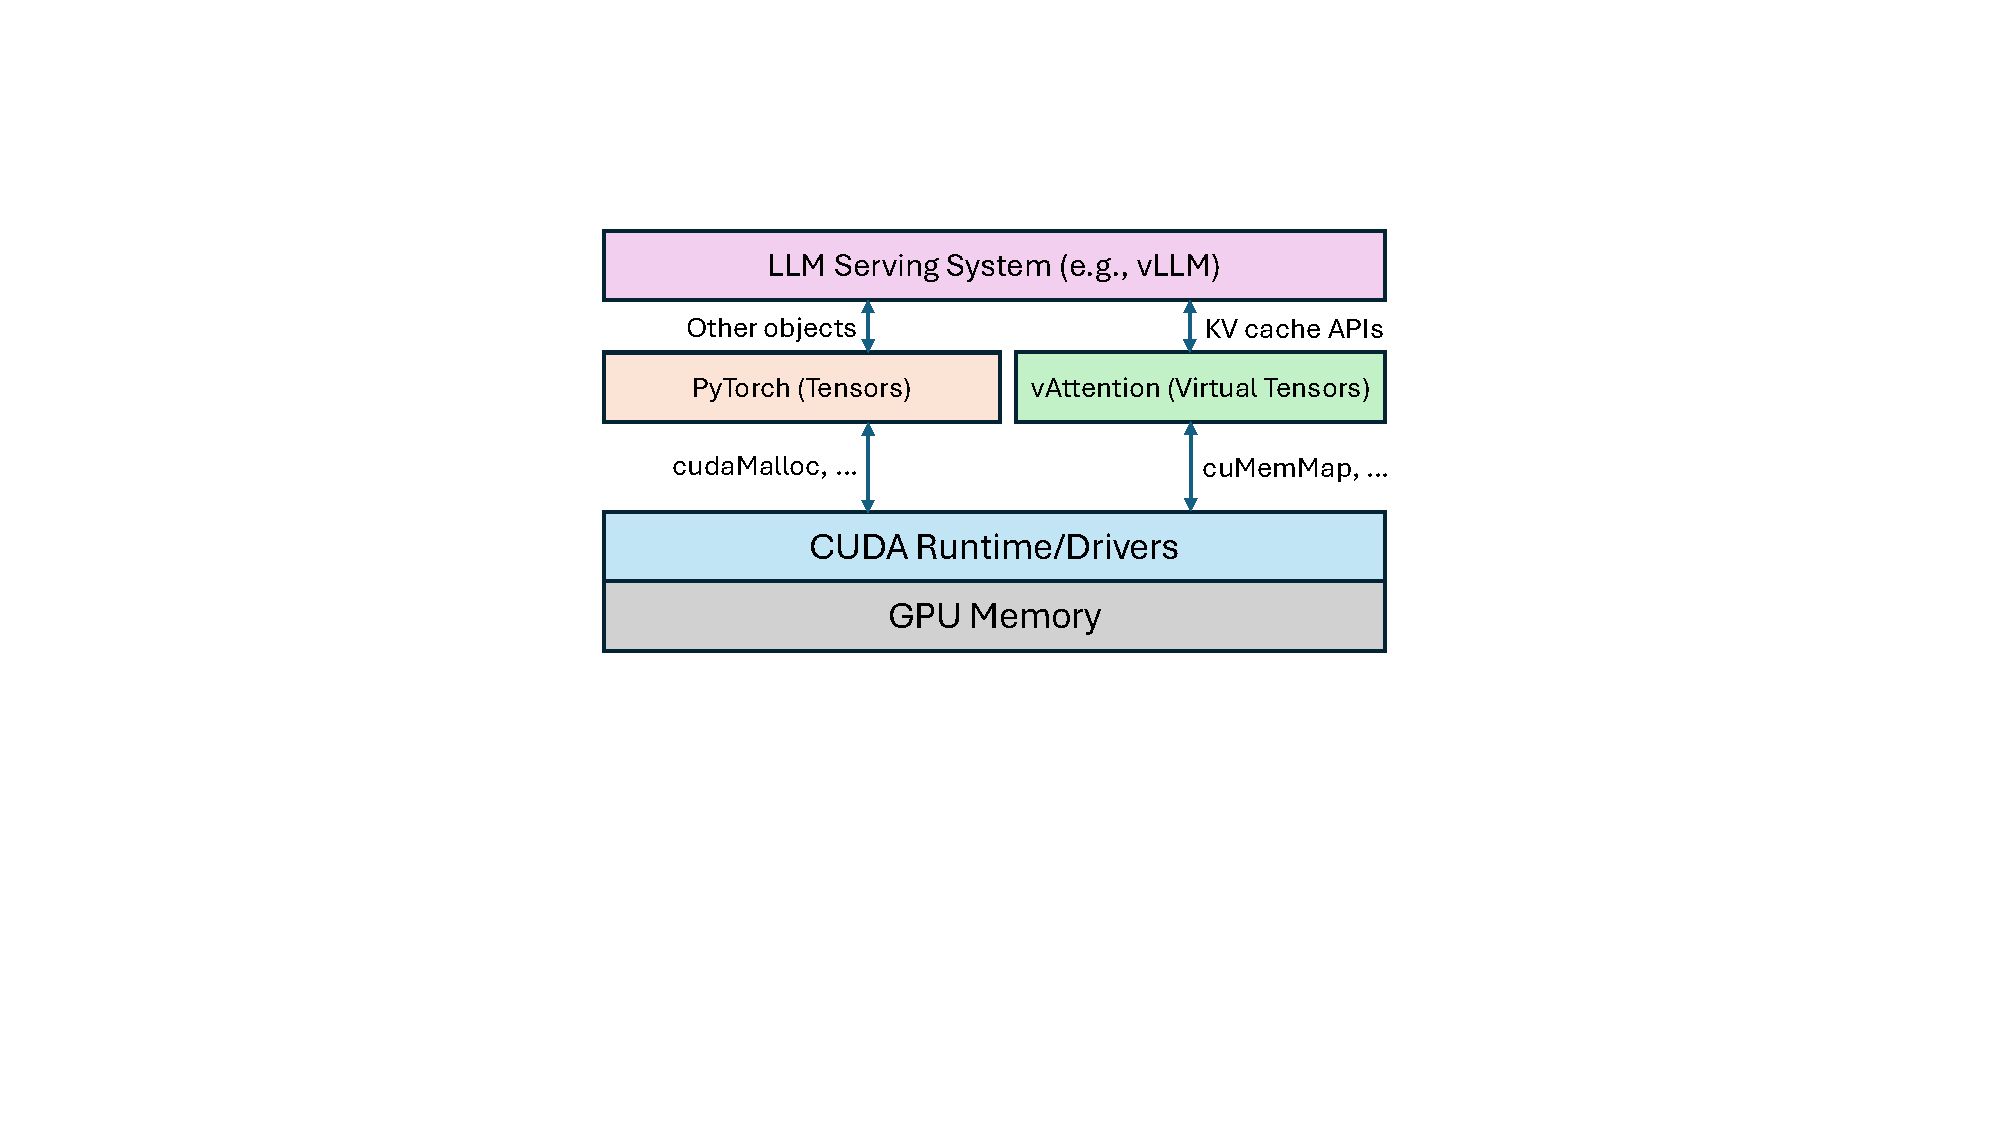
\includegraphics[trim={250 225 250 110}, clip=true, width=0.8\columnwidth]{figures/vattn.pdf}
    \caption{An LLM serving system interacts with \sysname for \kvcache management with a set of simple APIs listed in~\autoref{tab:design:vattn-apis}. All other memory objects (e.g., activations) are allocated by the standard PyTorch caching allocator.}
    \label{fig:design:vattn-usage}
\end{figure}


\subsubsection{Extending PyTorch caching allocator} \kvcache is a collection of tensors. In current deep learning frameworks such as PyTorch, a tensor allocated via APIs such as \torchempty comes with pre-allocated physical memory. This is because the PyTorch caching allocator relies on the \cudamalloc interface (\autoref{fig:design:vattn-usage}). Relying on the low-level API support from CUDA, we extend the PyTorch caching allocator to allow an application to reserve a virtual memory buffer for a tensor without committing physical memory ahead-of-time. We refer to tensors allocated via these APIs as virtual tensors.

\subsubsection{Request-level \kvcache indexing} A virtual tensor represents the \kcache (or \vcache) of a layer for the maximum batch size B. In these tensors, different requests occupy different non-overlapping sub-regions (say sub-tensors). We locate the sub-tensor of a request with a unique integer identifier \reqid that lies in the range of $0$ to $B-1$ (note that at most $B$ requests run simultaneously). The \kcache (or \vcache) offset of a request's sub-tensor in the virtual tensor of the entire batch is $\reqid\times S$ where $S$ is the maximum size of per-layer \kcache (or \vcache) of a request on a worker. The request identifier \reqid is allocated by \sysname.

\begin{table}[t!]
    \centering
    \scalebox{0.85}{
    \begin{tabular}{r|p{7cm}}
       \textbf{APIs}  & \textbf{Description} \\ \toprule
      \vattninit  & Initializes \sysname  with model parameters. \\ 
      & arguments: $N, B, L, H, D, P$, \texttt{page-group-size}. \\
      & return value: a list of \kvcache tensors.   \\ \hline
      \vattnallocid & Allocates an unused \reqid and marks it active \\
      & arguments: None \\
      & return value: an integer \reqid \\ \hline
      \vattnfreeid &  Frees a \reqid and marks it inactive \\
      & arguments: an integer \reqid \\
      & return value: None \\ \hline
      \vattnstep & Ensures \kvcache tensors are backed by physical pages up to the current context length of each active request  \\
      & arguments: an array of size B containing sequence lengths of each \reqid \\
      & return value: 0 (success), -1 (failure).\\
       \bottomrule
    \end{tabular}}
    \caption{Key APIs that \sysname exposes to a serving framework for dynamic \kvcache memory management.}
    \label{tab:design:vattn-apis}
\end{table}


\subsection{Serving LLMs with \sysname}
\label{sec:design:serving-llms}

We build \sysname as a Python library that internally uses a CUDA/C++ extension for interacting with CUDA drivers. Our library exposes a set of simple APIs to the serving framework (shown in~\autoref{fig:design:vattn-usage},~\autoref{tab:design:vattn-apis} and Algorithm~\autoref{alg:design:integration}). For simplicity, we discuss the use of these APIs from a single worker's perspective; all workers behave the same.


\subsubsection{Initial setup} When the serving framework starts, each model worker loads the \sysname library and configures it with model parameters $N, H, D, P$, $B$ and a preferred {\it page-group size} (\autoref{sec:opt:frag}) via the \vattninit API (line 4 in Algorithm~\autoref{alg:design:integration}). Internally,  \sysname reserves $2\times N$ virtual tensors on the worker, as shown in \autoref{fig:design:vattention}(a),  where $N$ is the number of layers hosted by the worker. These virtual tensors are reserved for the lifetime of the serving application. In addition, \sysname also pre-allocates physical memory pages at each worker during initialization. However, these pages are not mapped into the \kvcache at this point.


\begin{algorithm}[t]
%\begin{algocolor}
\caption{Using \sysname in a serving framework.}
\label{alg:design:integration}
\begin{algorithmic}[1]
\State \textnormal{max\_batch\_size $\gets$ B}
\State \textnormal{cache\_seq\_len $\gets$ [0]*B}
\State \textnormal{req\_batch\_idx $\gets$ dict()}
\State \textnormal{\underline{vattention.init(config\_params)}}
\While{\textnormal{!request\_pool.is\_empty()}}
    \For{\textnormal{$R_i$ in new\_requests}}
        \If{\textnormal{can\_schedule($R_i$)}}
            \State \textnormal{idx $\gets$ \underline{vattention.alloc\_reqid()}}
            \State \textnormal{req\_batch\_idx[$R_i$] $\gets$ idx}
            \State \textnormal{cache\_seq\_len[idx] $\gets$ prompt\_len($R_i$)}
        \EndIf
    \EndFor
    \State \textnormal{\underline{vattention.step(cache\_seq\_len)}}
    \State \textnormal{model.forward()}
    \For{\textnormal{$R_i$ in active\_requests}}
        \State \textnormal{idx $\gets$ req\_batch\_idx[$R_i$]}
        \If{\textnormal{is\_complete($R_i$)}}
            \State \textnormal{cache\_seq\_len[idx] $\gets$ 0}
            \State \textnormal{\underline{vattention.free\_reqid(idx)}}
        \Else
            \State \textnormal{cache\_seq\_len[idx] $+=$ 1}
        \EndIf
    \EndFor
\EndWhile
\end{algorithmic}
%\end{algocolor}
\end{algorithm}

\subsubsection{Scheduling a new request} When a new request is scheduled for the first time, the serving framework obtains a new \reqid from \sysname via \vattnallocid (line 8). All subsequent memory management operations of the request are tagged with this \reqid.



\subsubsection{Model execution} Before scheduling a batch for execution, the framework needs to ensure that the \kvcache sub-tensors of each active request are backed by physical memory (\autoref{fig:design:vattention}(b) and (c)). For this purpose, before dispatching the first kernel of an iteration to the GPU, the framework invokes the \vattnstep API (line 13), specifying the current context length of each request (context length is set to 0 for each inactive \reqid). Internally, \sysname ensures that enough physical pages are mapped for each active \reqid before returning execution back to the framework. If \sysname cannot satisfy the memory demand, it returns with a failure in response to which a serving framework can preempt one or more requests to allow forward progress (this is similar to \vllm's default behavior). We leave more sophisticated policies such as swapping out \kvcache to CPU memory as future work.



Depending on whether a request is in the prefill phase or decode phase, different amount of physical memory may need to be mapped for a given iteration. The prefill phase processes the input tokens of a given prompt in parallel. Therefore, the amount of physical memory needed to be mapped depends on the number of prompt tokens being scheduled. If the total \kcache size of all prompt tokens at one layer of the model is $s$ and page-group size is $t$, then each worker needs to ensure that at least $(s+t-1)/t$ page-groups are mapped in each of the $2\times N$ \kvcache sub-tensors of the given \reqid. 


For a request in the decode phase, the number of new page-groups required is at most one per virtual tensor. This is because each iteration produces only one output token for a request. \sysname internally tracks the number of page-groups mapped for each request and maps new page-groups only when prior page-groups are about to be exhausted. 


\subsubsection{Request completion} A request terminates when it reaches user specified or the maximum context length supported by the model, or when the model produces a special end-of-sequence token. The framework notifies \sysname  of a request's completion with \vattnfreeid (line 19). Internally, \sysname may unmap the physical pages of a completed request or defer them to be freed later (\autoref{sec:opt:defer}).


\noindent
\textbf{Supporting continuous batching:} Continuous batching poses one challenge in computing attention in our design. When a request from somewhere in the middle of a batch exits, it creates an unused hole in the virtual tensors of \kvcache. This layout is not supported by implementations that expect the query (Q) and \kvcache to be of the same size in batch ($B$) dimension. However, FlashAttention provides rich API support to address this issue; its argument \texttt{cache\_batch\_idx} allows Q and \kvcache to have different batch sizes and also be arranged in arbitrary order (i.e., batch index 0 in Q can be mapped to batch index 1 in \kvcache). \sysname benefits from this API support in terms of both performance and ease of programming; when the request composition of a batch changes, we update \texttt{cache\_batch\_idx} of running requests such that their Q tensors map to their respective \kvcache based on their \reqid.






